\documentclass[11pt,a4paper]{article}

\usepackage{style2017}
\newcounter{numexo}
\setcellgapes{1pt}

\begin{document}


\begin{NSI}
{Activité}{Les opérateurs logiques}
\end{NSI}


\subsection*{\Large Introduction}
Dans le processeur  de l'ordinateur et d'autres composants électroniques, on a des transistors qui sont des semi-conducteurs. Ils ont la particularité de laisser passer ou non le courant électrique. \medskip

Il existe deux types de transistor : les PNP et les NPN. \medskip

En les associant, ils vont modifier les courants électriques et donc les valeurs des bits $0$ et $1$ qui représentent le courant électrique.\medskip

Cette activité se fait sur le logiciel \textbf{Logisim} qui permet de créer des circuits logiques.

Une fois connecté à votre session, aller sur le lecteur réseau $L:\backslash ro \backslash logisim$ puis lancer l'application Logisim.\bigskip

Le logiciel permet de construire des circuits avec des opérateurs logiques. Chaque circuit est composé:
\begin{itemize}
\item d'un ou plusieurs bits en entrée;
\item un seul bit de sortie;
\item un ou plusieurs opérateurs logiques;
\item de lien pour connecter les éléments.
\end{itemize}

Voici ci-dessous un exemple de circuit logique:

\begin{center}
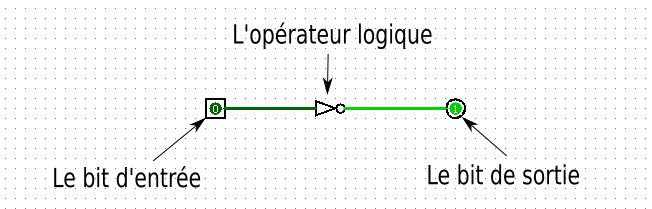
\includegraphics[scale=0.8]{img/presentation_element.png}
\end{center}

La construction d'un circuit logique se fait lorsque l'icône "flèche" est sélectionnée.

\subsection*{\Large L'opérateur logique NOT }
L'opérateur logique NOT est représenté symboliquement par:
\begin{center}
 
\includegraphics[scale=0.8]{img/operateurNOT.png}
 \end{center} 
\begin{enumerate}
\item Créer un circuit logique composé de l'opérateur NOT, d'une entrée et d'une sortie.

Représenter votre circuit ci-dessous.\vspace{1.5cm}
\item En cliquant sur l'icône "main", vous pouvez modifier la valeur du bit d'entrée. Observer alors la valeur du bit de sortie.
\item On note \textbf{A} le bit d'entrée. Le bit de sortie se note alors \textbf{NOT(A)}.
Compléter le tableau ci-dessous selon les valeurs prises par l'entrée \textbf{A}.

\begin{center}
\begin{tabular}{*{2}{|C{1.5cm}}|}\hline
A & NOT(A) \\\hline
 & \\
 & \\
 & \\
 & \\\hline
\end{tabular}
\end{center}


\end{enumerate}


\subsection*{\Large L'opérateur logique ET }

L'opérateur logique ET est représenté symboliquement par:
\begin{center}

\includegraphics[scale=0.8]{img/operateurET.png}
\end{center} 

\begin{enumerate}
\item Créer un circuit comprenant 2 entrées binaires, une porte logique \textbf{ET} et une sortie binaire.

Représenter votre circuit ci-dessous.\vspace{2cm}

\item Modifier la valeur des bits d'entrée et observer la valeur du bit de sortie.

\item On note \textbf{A} et \textbf{B} les bits d'entrée. Le bit de sortie se note alors \textbf{A ET B}. Compléter la table ci-dessous:

\begin{center}
\begin{tabular}{*{2}{|C{1cm}}|C{1.6cm}|}\hline
$A$ & $B$ & $A \text{~ET~} B$ \\\hline
 & & \\
 & & \\
 & & \\
  & & \\
 & & \\
 & & \\\hline
\end{tabular}
\end{center}
\end{enumerate}




\subsection*{\Large L'opérateur logique OU }
L'opérateur logique OU est représenté symboliquement par:
\begin{center}

\includegraphics[scale=0.8]{img/operateurOU.png}
\end{center} 

\begin{enumerate}
\item Créer un circuit comprenant 2 entrées binaires, une porte logique \textbf{OU} et une sortie binaire.

Représenter votre circuit ci-dessous.\vspace{2cm}

\item Modifier la valeur des bits d'entrée et observer la valeur du bit de sortie.

\item On note \textbf{A} et \textbf{B} les bits d'entrée. Le bit de sortie se note alors \textbf{A OU B}. Compléter la table ci-dessous:

\begin{center}
\begin{tabular}{*{2}{|C{1cm}}|C{1.6cm}|}\hline
$A$ & $B$ & $A \text{~OU~} B$ \\\hline
 & & \\
 & & \\
 & & \\
  & & \\
 & & \\
 & & \\\hline
\end{tabular}
\end{center}
\end{enumerate}




\newpage


\subsection*{\Large Circuit logique 1}

On veut créer un circuit avec trois entrées binaires A, B et C représentant l'expression logique A ET B OU C.

\begin{enumerate}
\item Créer un circuit logique pour cette expression et le représenter ci-dessous. \vspace{3cm}

\item Modifier la valeur des bits d'entrée et observer la valeur du bit de sortie.

\item Construire un tableau contenant toutes les valeurs possibles en entrée et la valeur en sortie. On pourra insérer des colonnes pour des valeurs intermédiaires. \vspace{5cm}
\end{enumerate}




\subsection*{\Large Circuit logique 2}

On donne le circuit logique avec trois entrées binaires A, B et C.

\begin{center}
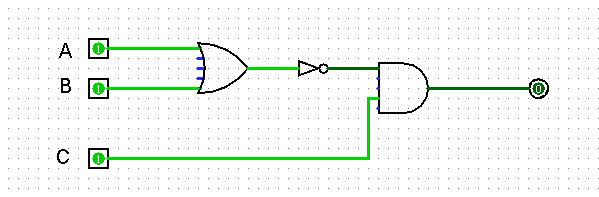
\includegraphics[scale=0.8]{img/circuit2.png}
\end{center}

\begin{enumerate}
\item Reproduire ce circuit puis modifier la valeur des bits d'entrée et observer la valeur du bit de sortie.

\item Proposer une expression logique associée à ce circuit.

\item Construire un tableau contenant toutes les valeurs possibles en entrée et la valeur en sortie. On pourra insérer des colonnes pour des valeurs intermédiaires. \vspace{5cm}
\end{enumerate}



\end{document}